\documentclass{article}

\usepackage[a4paper,left=18mm,right=18mm,top=20mm,bottom=18mm]{geometry}
\usepackage[italian]{babel}

\usepackage{titling}
\usepackage{graphicx}
\usepackage{subcaption}
\usepackage{float}

\title{Considerazioni sul dataset di SCG }
\author{Ianitchii Alin, Gabriele Marchesi, David Guzman Piedrahita e Marco Vinciguerra}
\date{\today}    

\begin{document}
\maketitle
\begin{enumerate}
    \item \textbf{Tassi di cambio} $\rightarrow$ contiene i tassi di cambio sia a BUDGET che a CONSUNTIVO
    \item \textbf{Impiego orario risorse} $\rightarrow$ contiene articoli (colonna nr articolo) non unique. 
    \\Considerazione = ordine di produzione $\rightarrow$ prima c’è budget e poi consuntivo, sempre. Il controllo qualità viene eseguito sempre dopo nell’ordine di produzione. ART0000128 ha solo controllo di qualità.
    Controllo qualità ha sempre tempo di risorsa nullo. Fresatura ha quantità di output = 0.
    \item \textbf{Vendite} $\rightarrow$ la colonna Nr.Origine corrisponde all’id del cliente.
    \item \textbf{Consumi} $\rightarrow$ consumo di materia prima. Nr.documento $\rightarrow$ si riconduce all’ordine di produzione.
    \\Possibile camino di join $\rightarrow$ doppio join con la tabella impiego orario risorse.
    \item \textbf{Costo orario risorse} $\rightarrow$ Contiene il codice della risorsa e il costo orario della risorsa.
    \item \textbf{Clienti} $\rightarrow$ c’è il codice cliente e la valuta.
\end{enumerate}
\section{Considerazioni}
\textbf{N.B:} Non c’è corrispondenza biunivoca tra budget e consuntivo.
\\\textbf{N.B:} Per ogni ordine di produzione nella tabella dei costi possono corrispondere più NrArticolo
\\\textbf{ASSUNZIONI:} Nella tabella "Impiego orario risorse" si assume che quando la quantità di output è 0 significa che è un processo che non è terminato in giornata (come ad esempio il 
processo di fresatura) e si è deciso di unire le due righe facendo la somma delle risorse.
\\\textbf{N.B:} Già a budget viene previsto che la stessa unità di materia prima viene comprata a prezzi differenti. Bisogna già vedere a consuntivo a quanto è stata acquistato
\\\textbf{N.B:} Uno stesso articolo può essere realizzato con materie prime differenti.
\\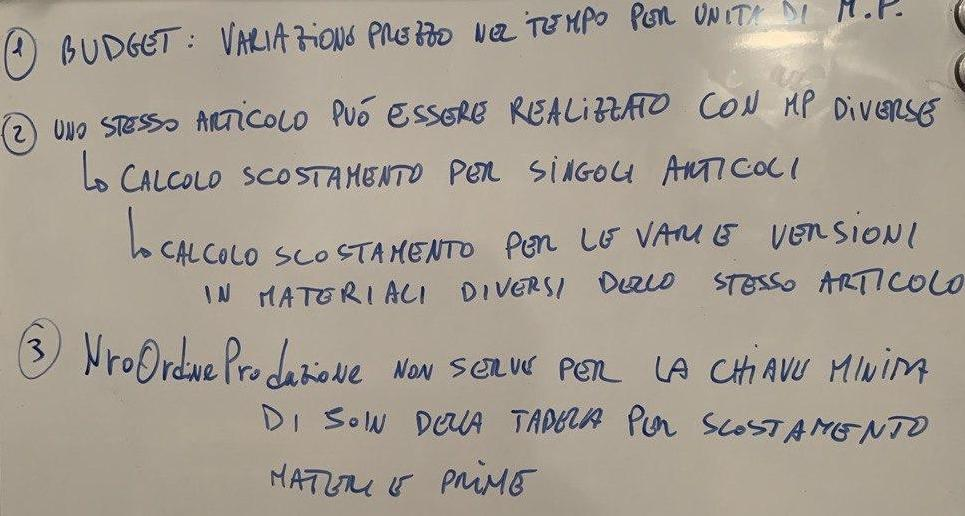
\includegraphics[scale = 0.4]{Lavagnetta.jpg}
\section{Formule matematiche}

$$QuantityOutput*\sum_{i}\frac{ImportoCostoTotale}{QuantityMPImpiegata_{i}}*QuantityMPImpiegata_{i}$$
\section{Possibili scostamenti dei costi}
\begin{itemize} 
    \item \textbf{Totale} \rightarrow  $Scostamento_{i}$ = Totale costi budget - Totale costi consuntivo
    \item \textbf{Materia prima} \rightarrow  $Scostamento_{i}$ = Costi budget $MP_{i}$ - Costi Consuntivo $MP_{i}$
    \item \textbf{Articolo} \rightarrow  $Scostamento_{i}$ = Costi Budget $MP_{i}$ - Costi Consuntivo $MP_{i}$
\end{itemize}

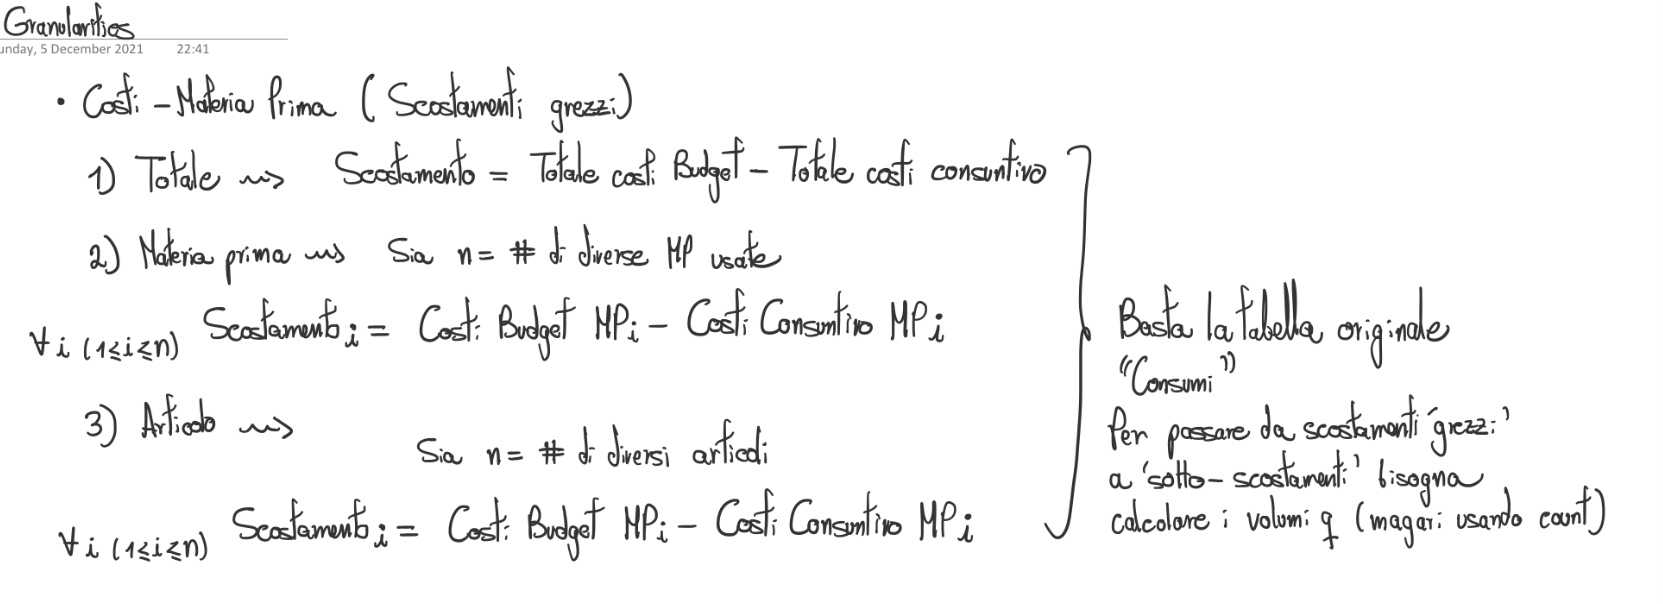
\includegraphics[scale = 0.25]{Scostamenti1.jpg}

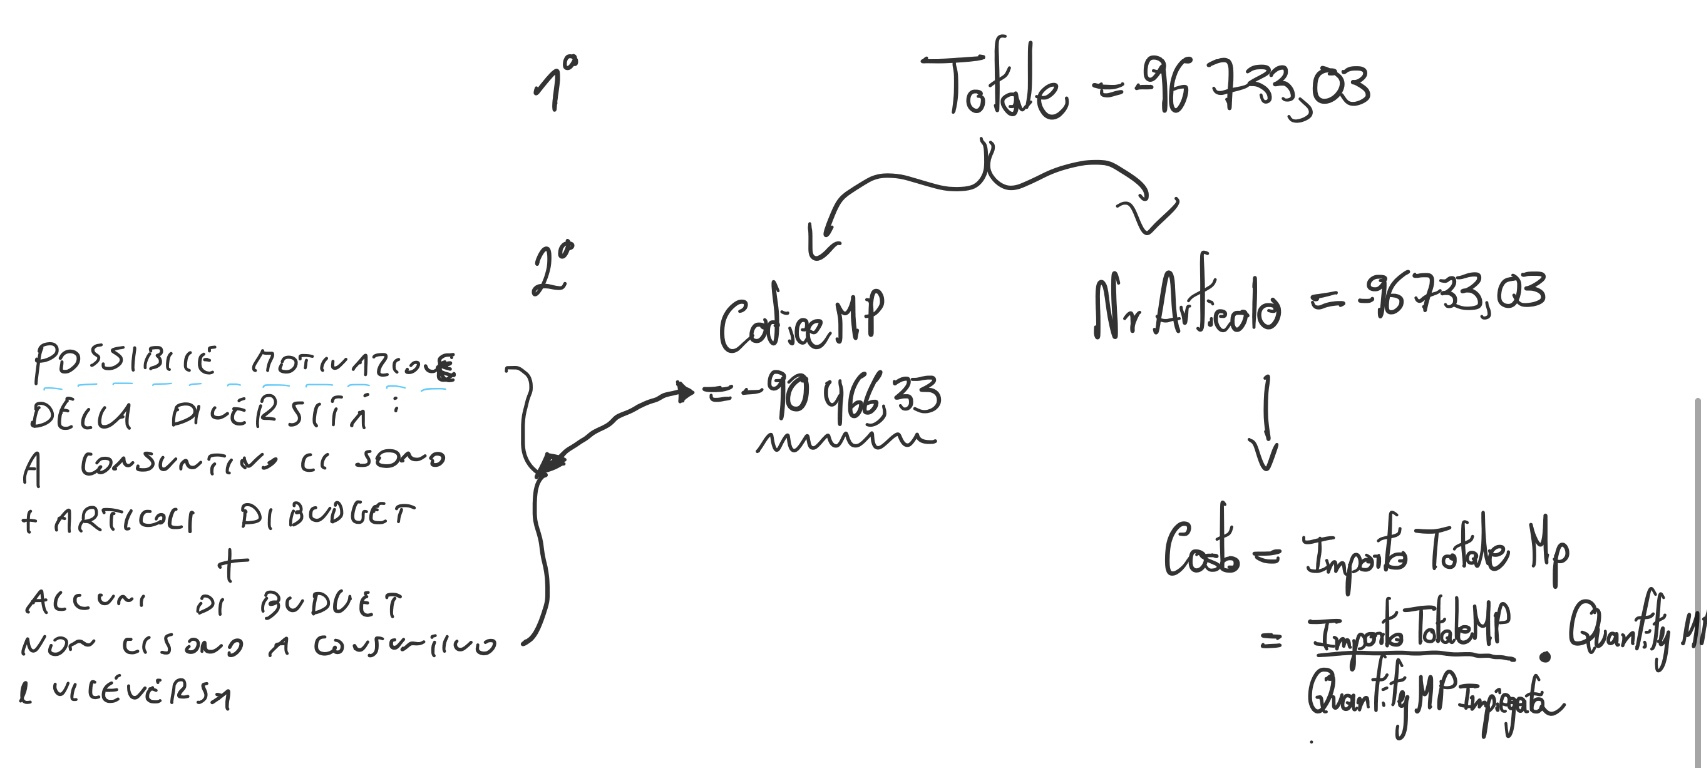
\includegraphics[scale = 0.25]{Scostamenti2.jpg}
\section{Possibili scostamenti delle vendite}
\begin{itemize}
\end{itemize}
\end{document}
